\section{Results}
\label{sec:Results}

In this section we present and describe the results for our methods with their variations. For this we use the previously introduced error measure, calculate it for all available fridges and summarise the results. We show the results as graphics for easier interpretation. The tables with the exact values are shown in the appendix. 

\subsubsection{History}
\label{sec:History}

As mentioned various times throughout this thesis, the length of the history is one of the parameters which can be adjusted. Since we deal with time series with different lengths, we take the history as a fraction of the total length. In figure \ref{fig:History Comp1} and \ref{fig:History Comp2} we visualise the results as a boxplot, a quantile plot and a histogram. 

\begin{figure}[htb]
\centering
\begin{subfigure}[b]{0.8\textwidth}
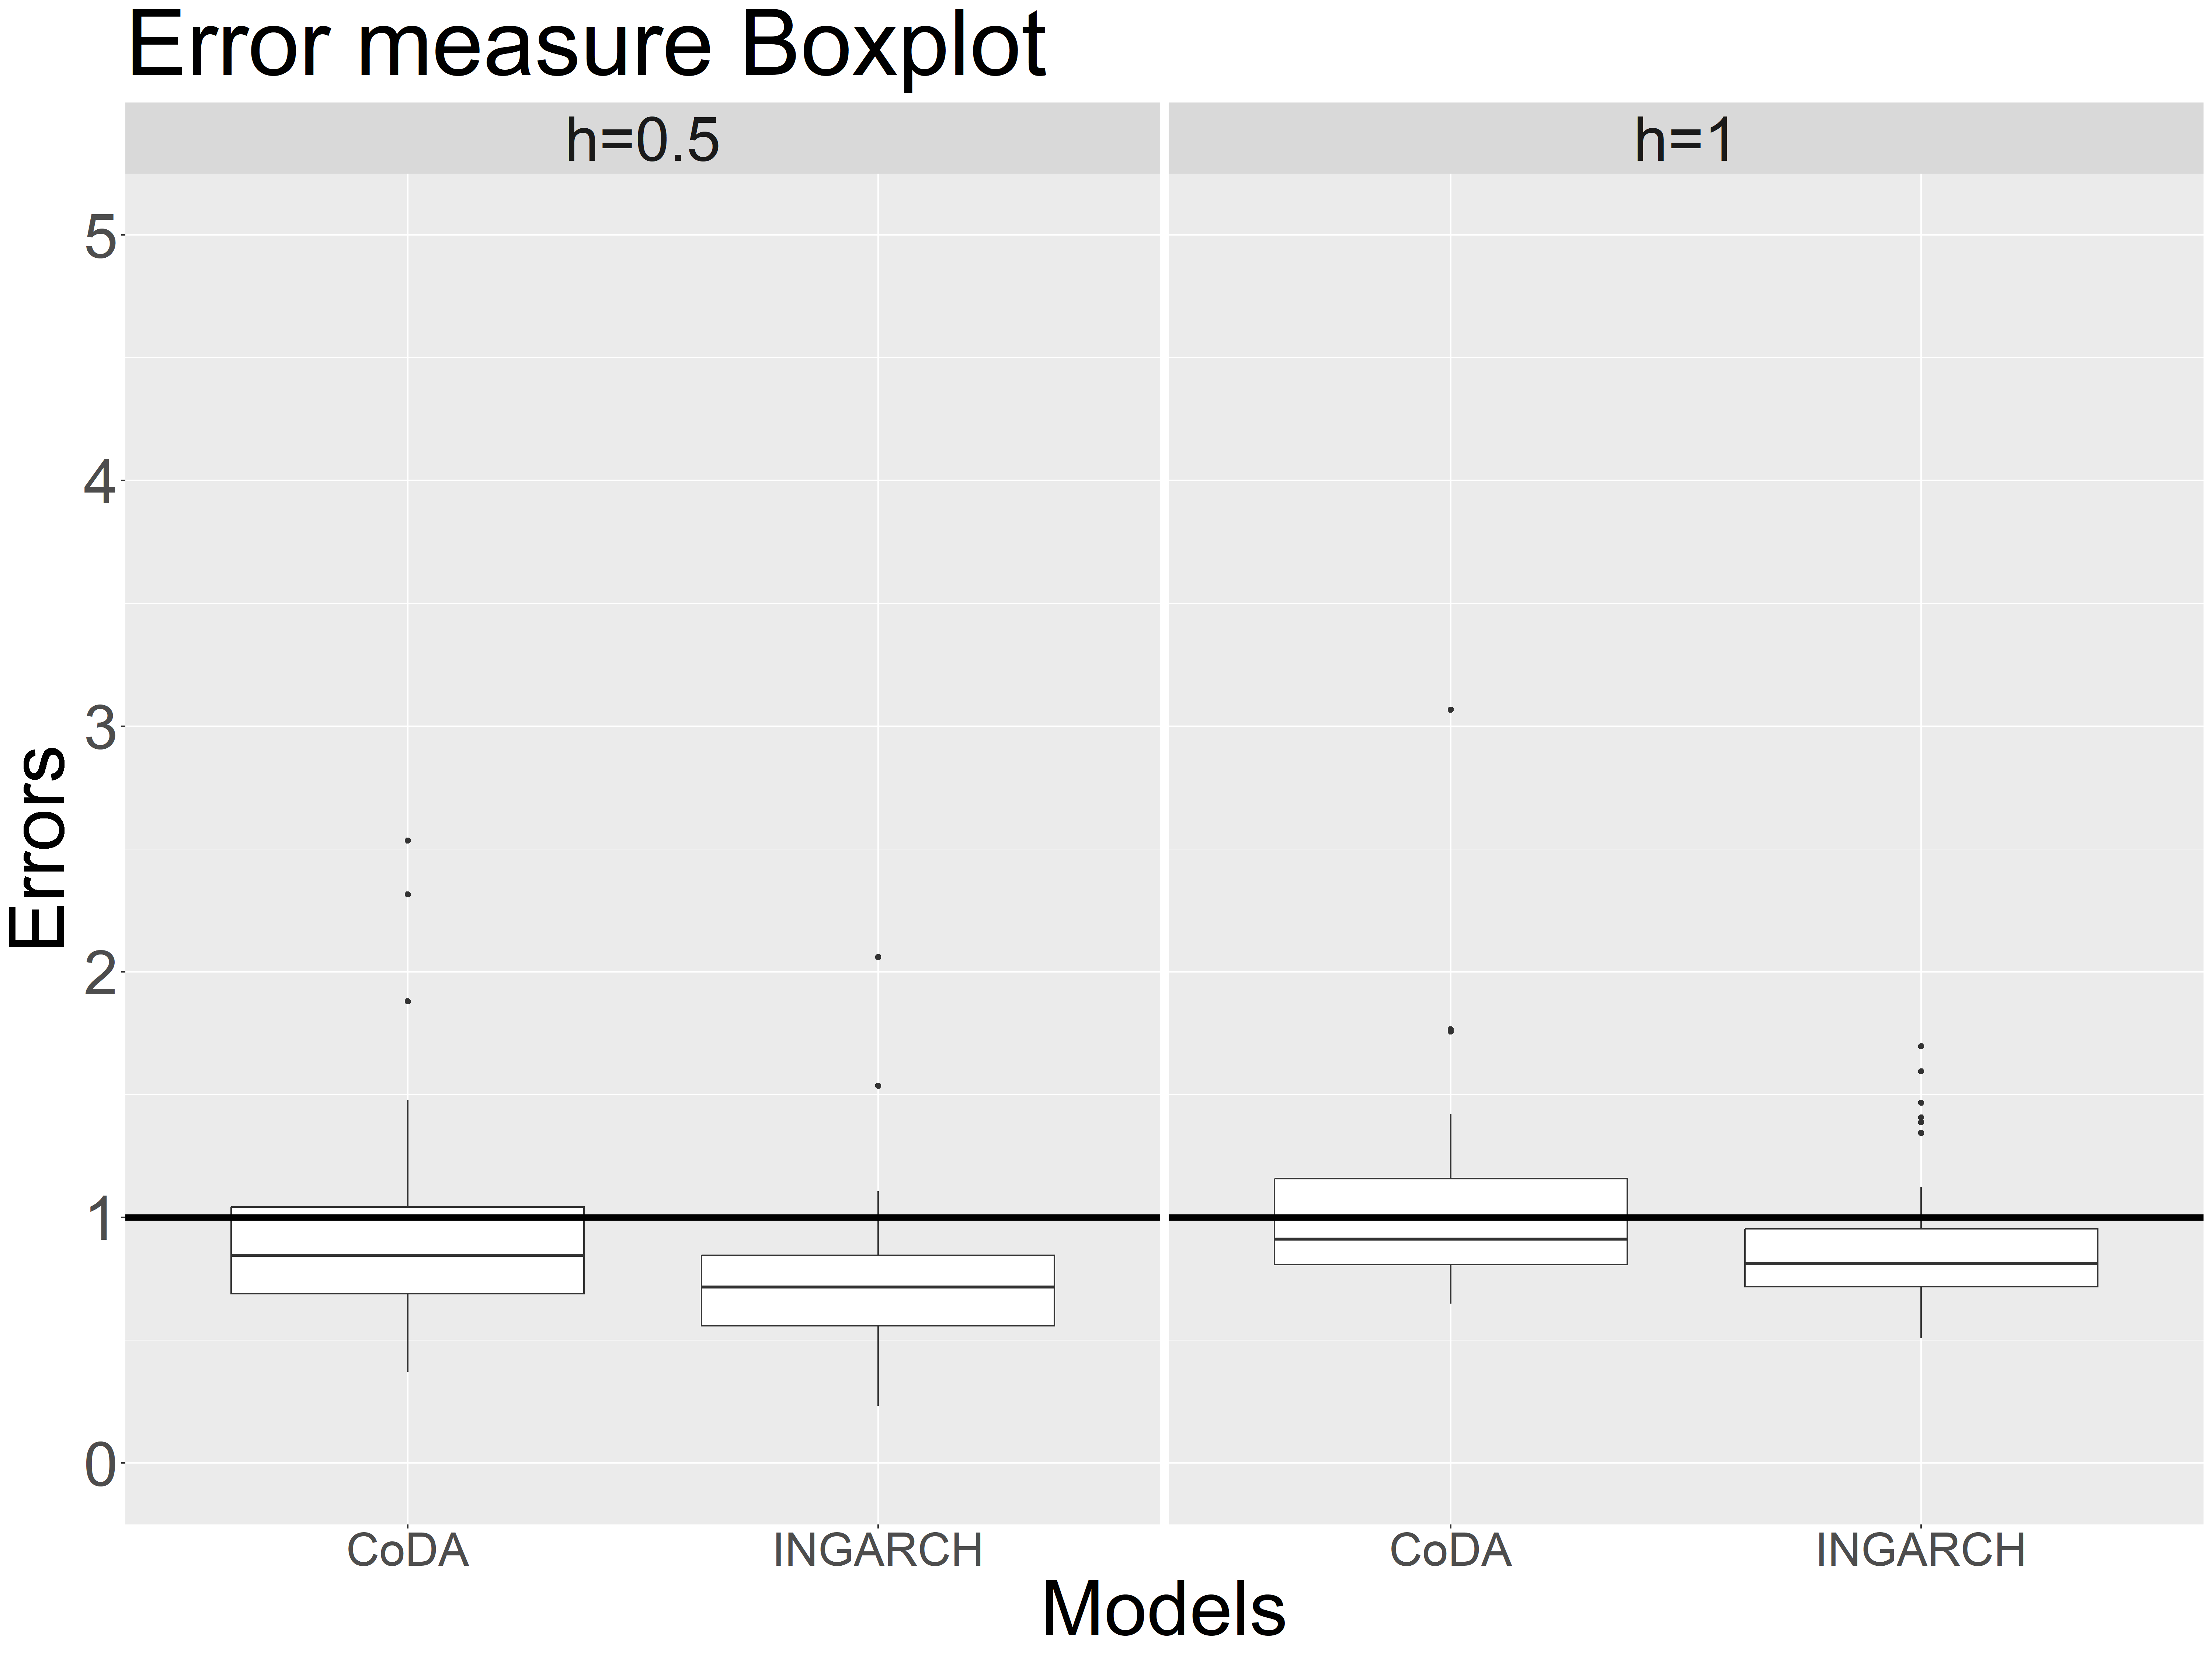
\includegraphics[width=\textwidth]{ErrorMeasureCombined_Box_all__Variation_history.png}
\caption{Boxplot for different history lengths}
\label{fig:History Box}
\end{subfigure}
\hfill
\begin{subfigure}[b]{0.8\textwidth}
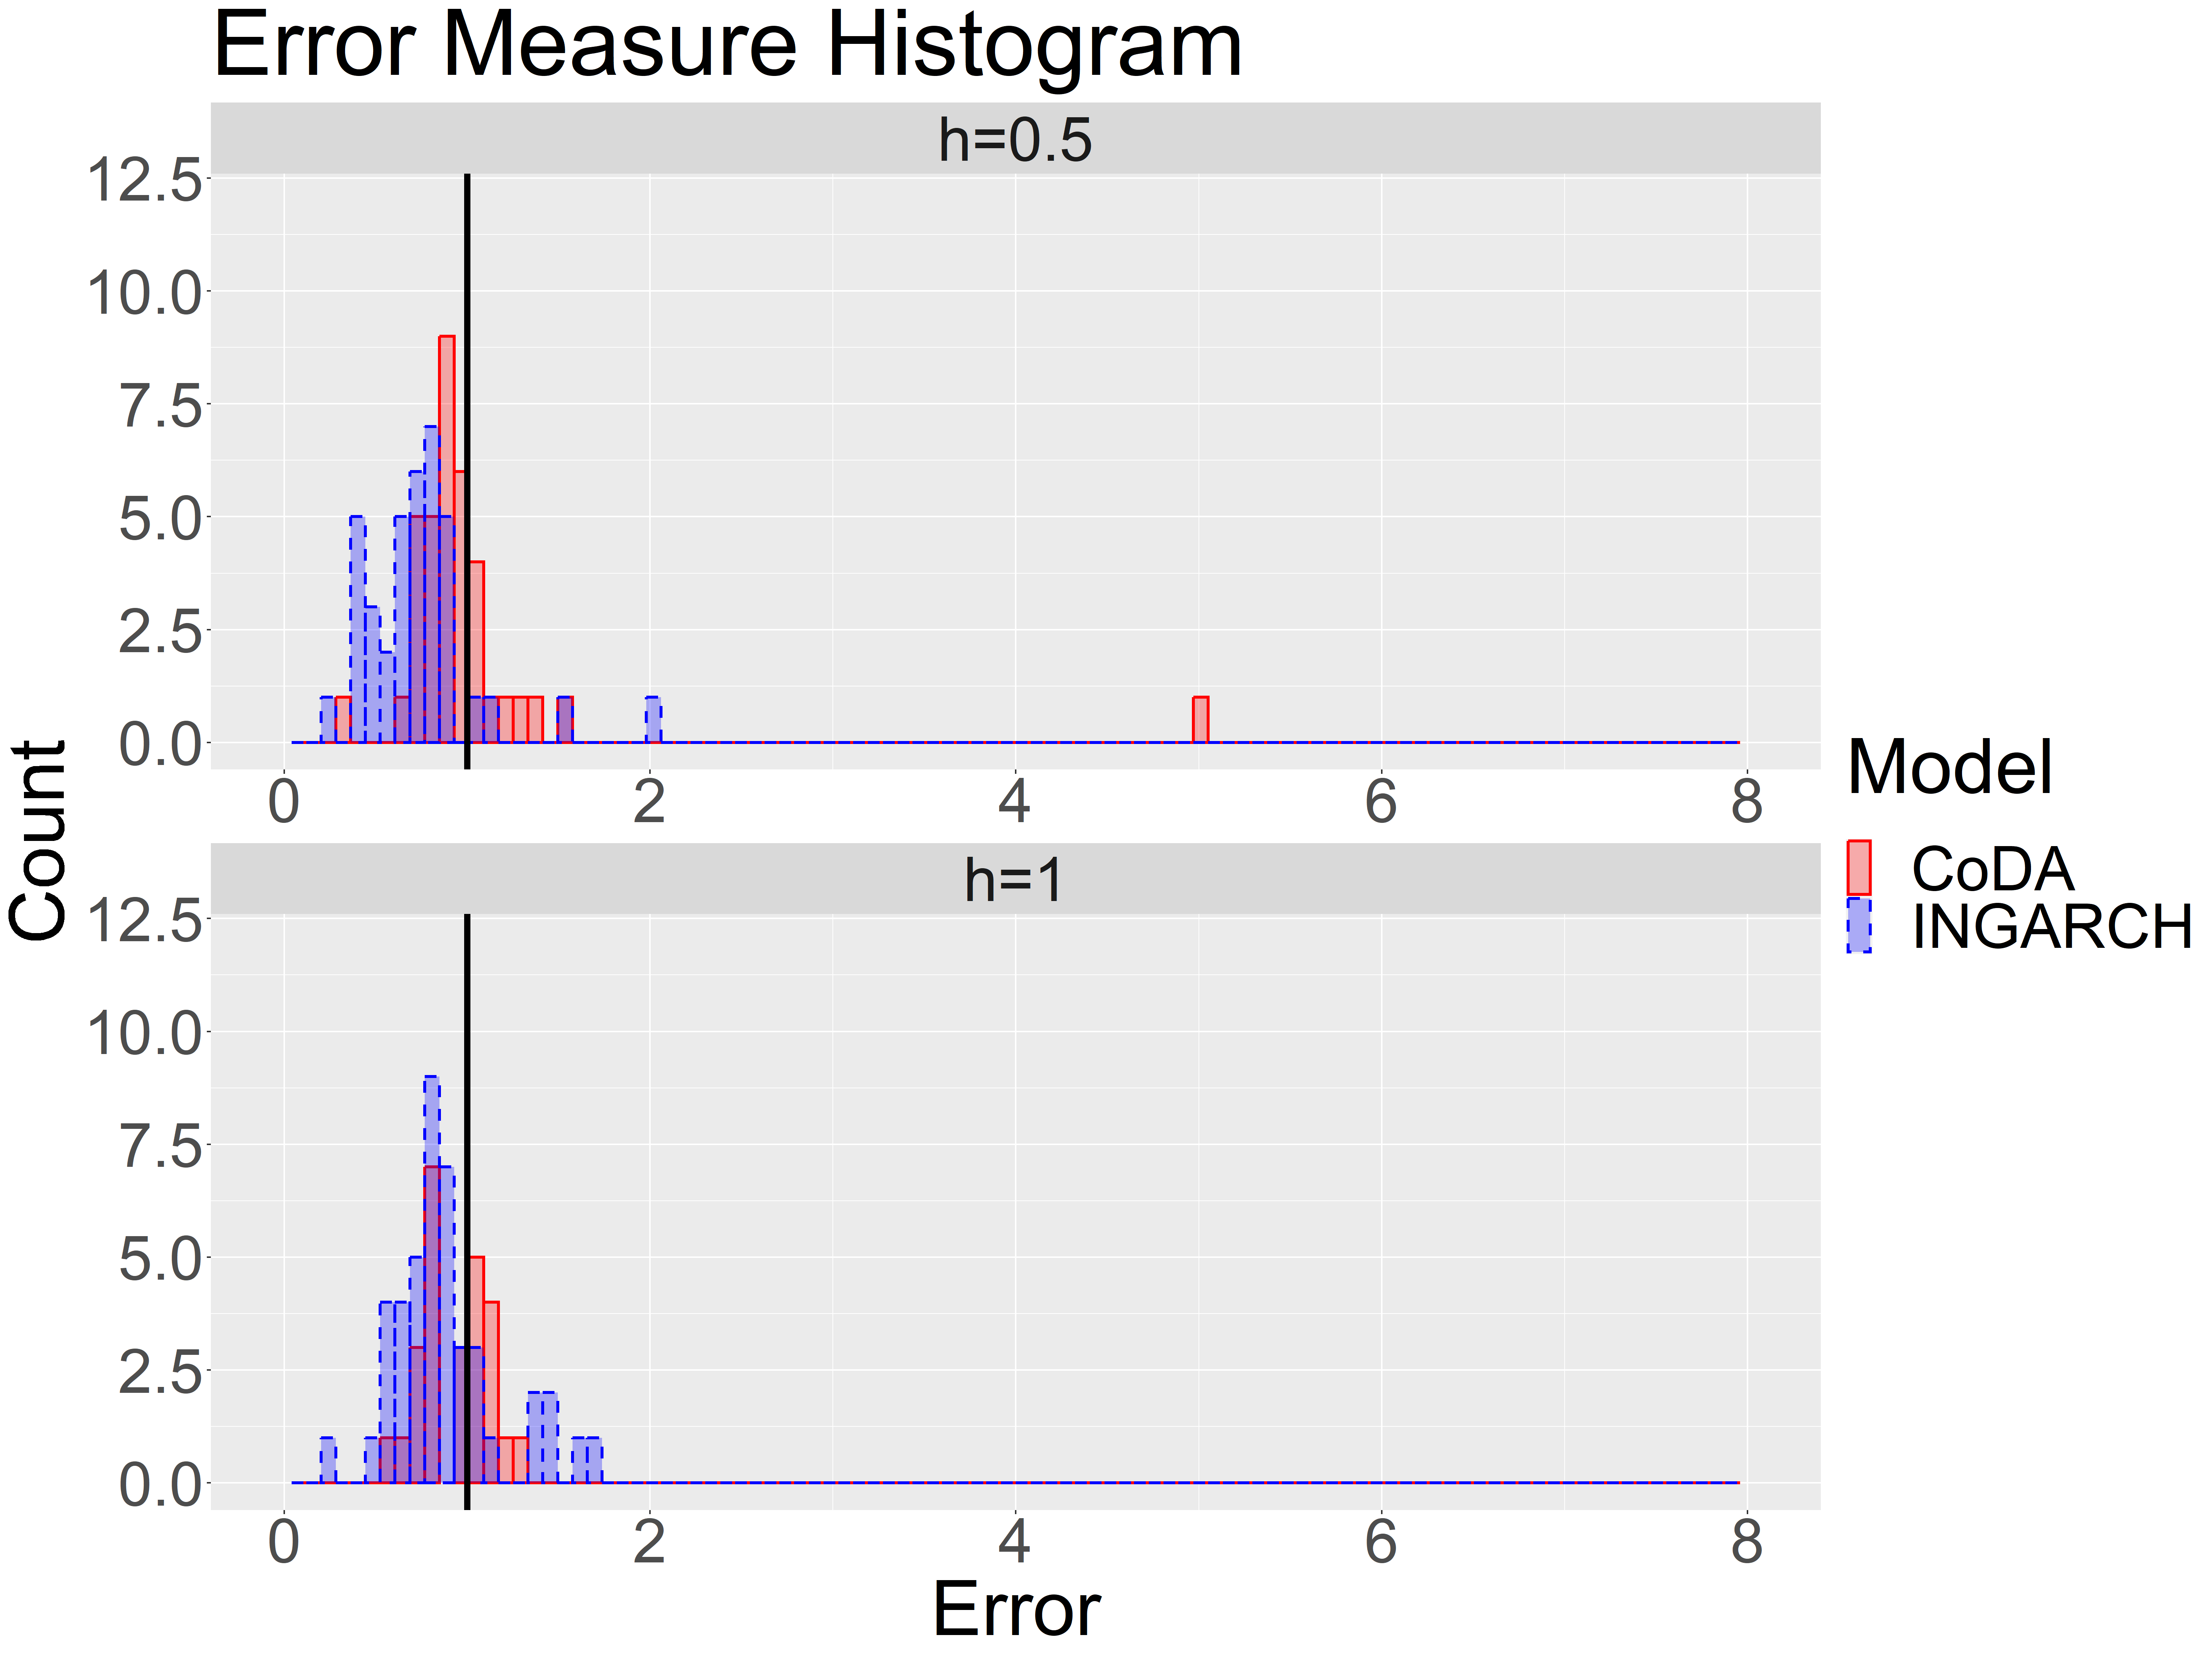
\includegraphics[width=\textwidth]{ErrorMeasureCombined_Histogram_all__Variation_history.png}
\caption{Histogram for different history lengths}
\label{fig:History Hist}
\end{subfigure}
\caption{Comparison of different history lengths}
\label{fig:History Comp1}
\end{figure}

\begin{figure}[htb]
\centering
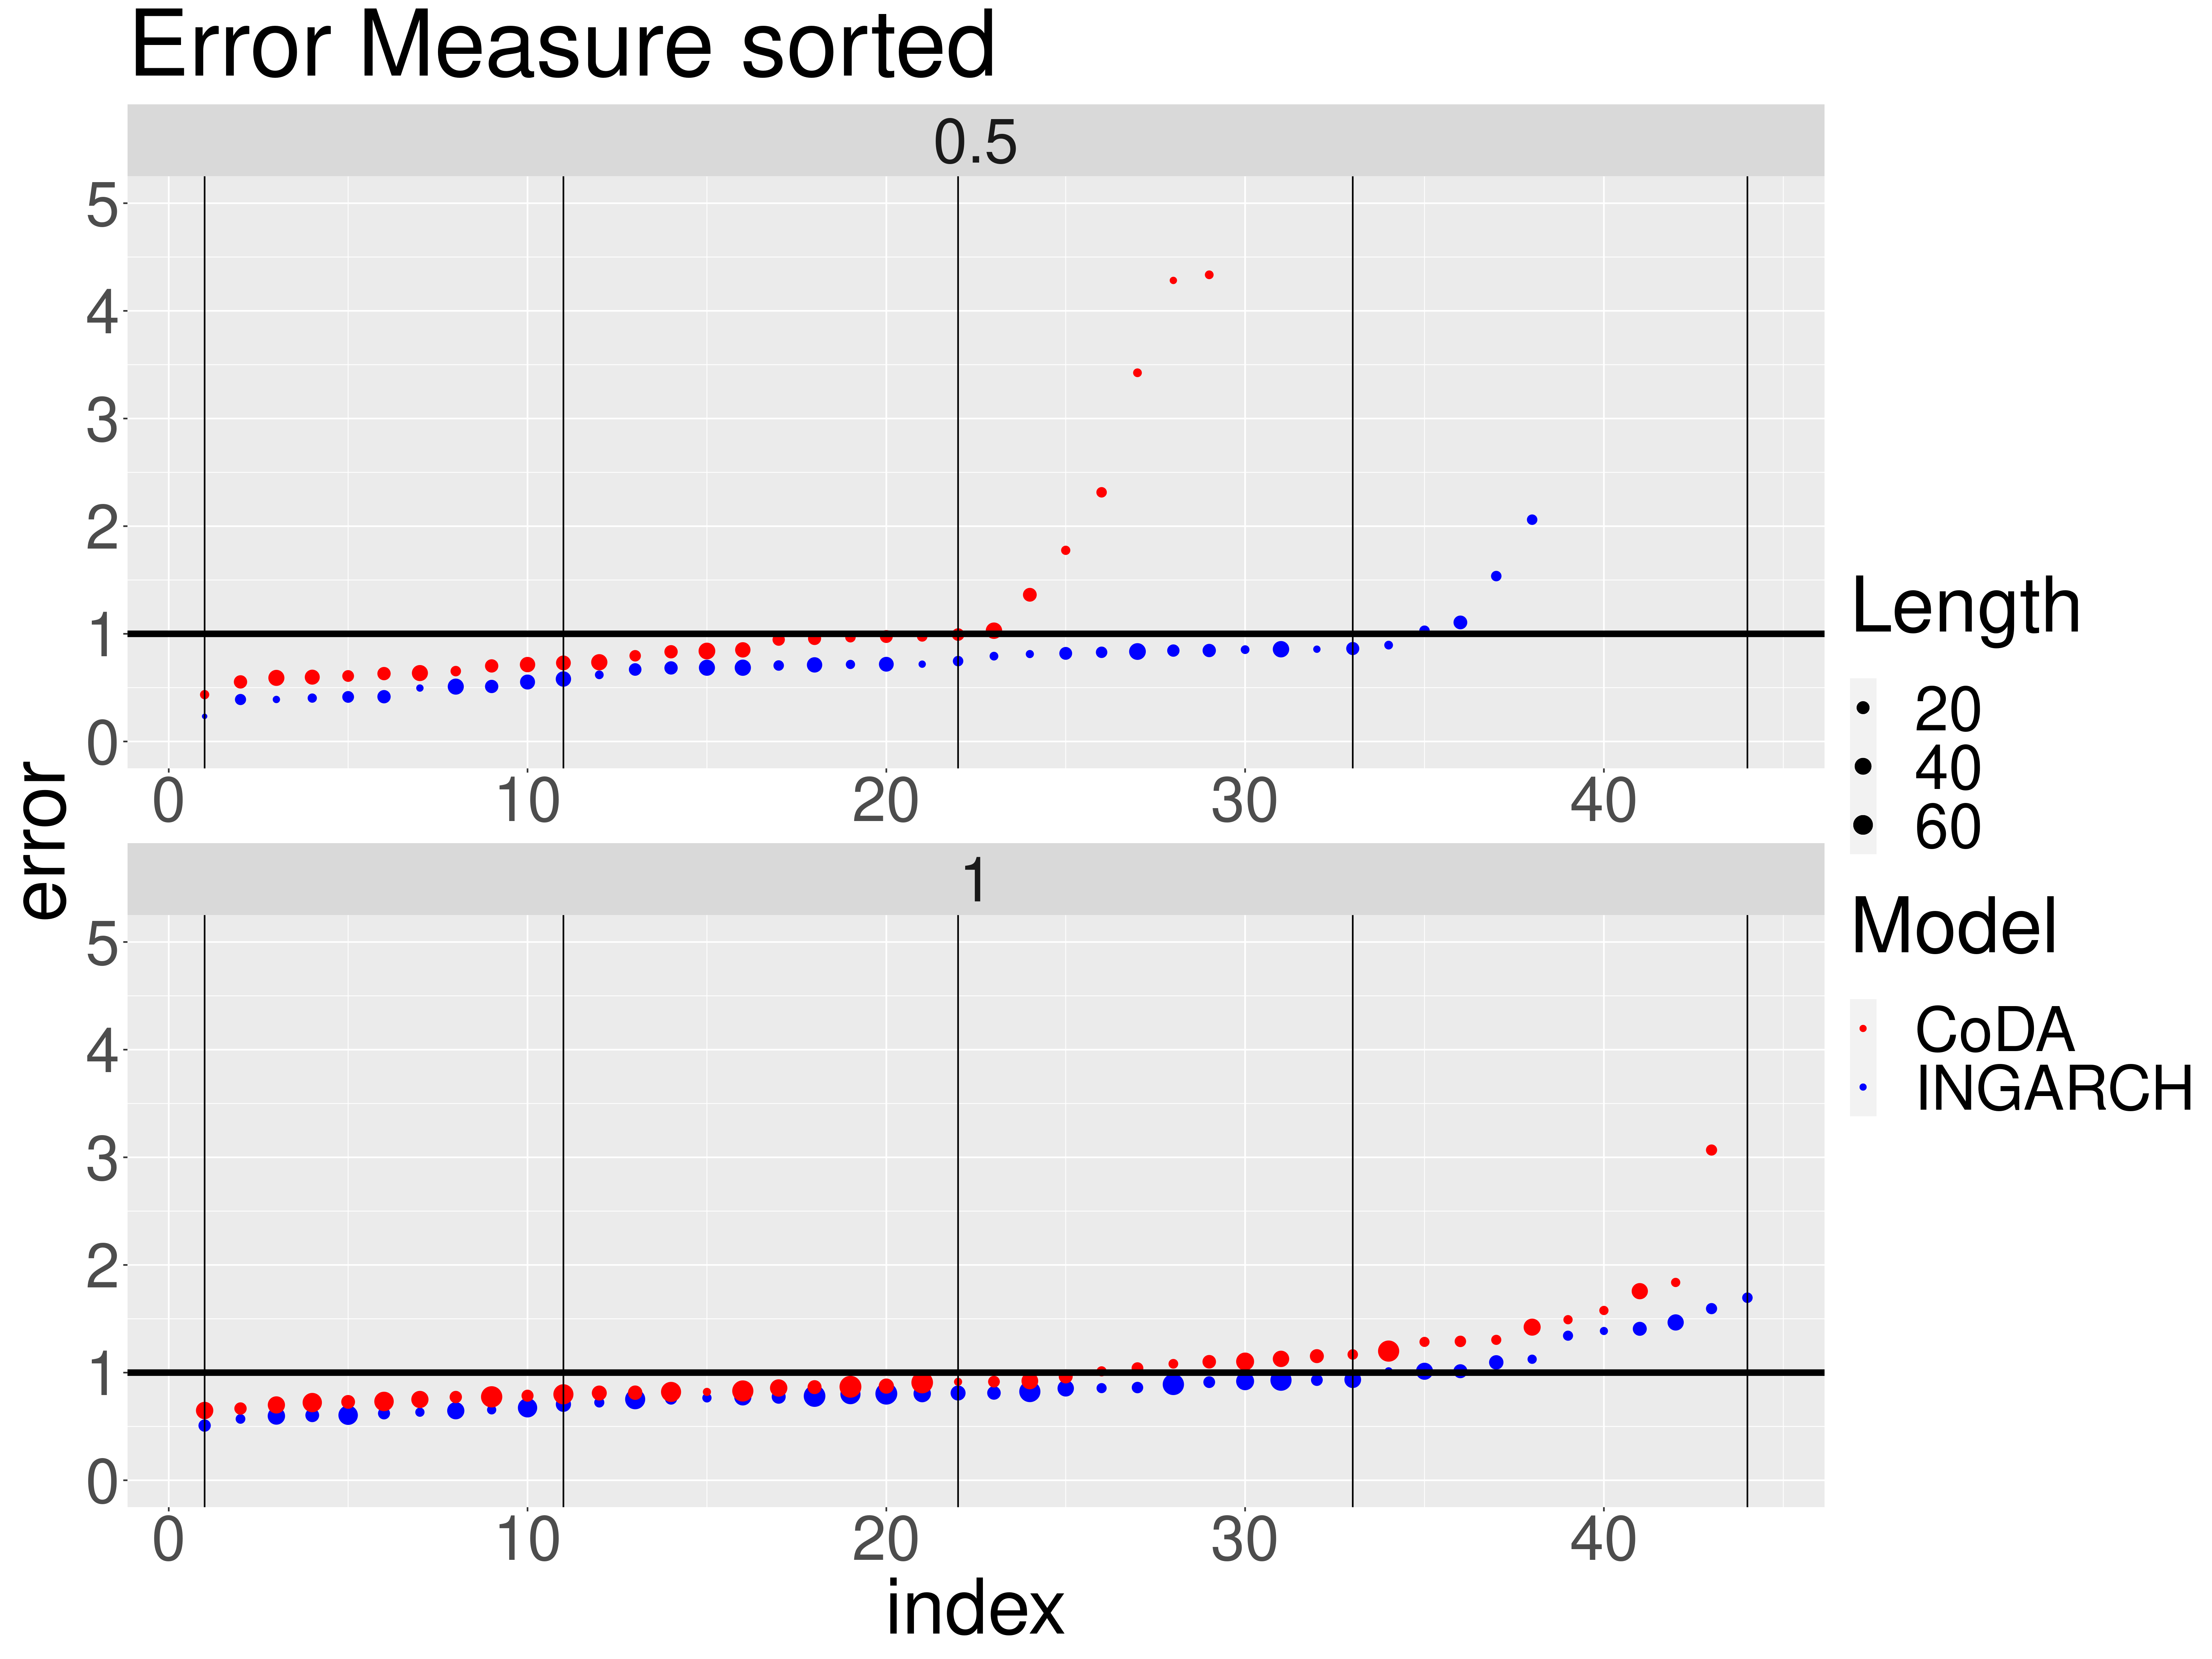
\includegraphics[width=0.8\textwidth]{ErrorMeasureCombined_Quant_all__Variation_history.png} 
\caption{Quantile Plot for different history lengths}
\label{fig:History Comp2}
\end{figure}

In figure \ref{fig:History Comp1} we can see that the results for CoDA vary for the different history lengths. While for a history of half of the length of the original time series, on around 75\% of the fridges the error measure is smaller than 1, this number drops to 50\% if we use the whole history. However, one can see in the quantile plot \ref{fig:History Comp2} that we have 8 less values for the factor 0.5 than for 1. This means that either we have larger values than the limits of the y-axis or that the method was unable to compute any result at all. 

For INGARCH, the results are very similar. For a factor of 1 we get slightly higher values for the error measure as seen in \ref{fig:History Comp1}. But again in \ref{fig:History Comp2} we see that we have less values for the shorter history. So again they are either too large to be shown, or there do not exist any values at all. 